% ----- Compile with LuaLaTeX! -----
% ----- Compilation requires the folders `fonts, figures' and a local LaTeX installation -----
\documentclass[12pt,twoside]{article}
\usepackage[all]{nowidow} %Single lines across page breaks are not allowed
\usepackage{graphicx} %Insertion of images
\graphicspath{{figures/}}
\usepackage[a4paper, margin=2.5cm, bottom=2cm,top=2cm]{geometry} %Page layout formatting
\usepackage{enumitem} %Bullet point formatting
\setlist[enumerate]{leftmargin=15pt}
\setlist[itemize]{leftmargin=15pt}
\usepackage{xcolor} %Custom colours
\usepackage{amsmath} %Alphabetical math variables
\usepackage{amssymb} %Math symbols
\usepackage{caption} %Caption formatting
\usepackage{subcaption} %Allows grouping multiple objects along with subcaptions for each
\usepackage{tabularx} %Table cell formatting
\usepackage{framed} %Creation of coloured domains
\usepackage{tocloft} %Table of Contents customization
\usepackage[normalem]{ulem} %Non-float underline and strikethrough
\usepackage{microtype} %Subtle typography improvements
\usepackage[hidelinks]{hyperref} %Creation of hyperlinks between document sections
\usepackage{cleveref} %Referencing adds the type of reference before its numbering in \autoref
\usepackage{titling} %Title page formatting
%Fonts and language settings
\usepackage{fontspec} %Setting up fonts per language script
\usepackage{polyglossia} %Language declaration commands
\usepackage[autostyle=true]{csquotes} %Language aware quotation

%Polyglossia settings: Each language separate in case options necessary
\setdefaultlanguage[variant=british]{english}
\setotherlanguage{korean}
\setotherlanguage{chinese}
\setotherlanguage{japanese}
\setotherlanguage{sanskrit}

%Font settings for fontspec
\defaultfontfeatures+{Path=fonts/, BoldFont=*-Bold, UprightFont=*-Regular, Extension = .ttf}
% Main Fonts (English)
\setmainfont{NotoSans}[
    Script = Latin,
    ItalicFont=*-Italic,
    BoldItalicFont = *-BoldItalic
]
\setsansfont{NotoSerif}[
    Script = Latin,
    ItalicFont=*-Italic,
    BoldItalicFont = *-BoldItalic
]
\setmonofont{NotoSansMono}[
    Script = Latin
]
% ------- Other fonts -------
% Devanagari (Sanskrit)
\newfontfamily\devanagarifont{NotoSansDevanagari}[
    Script = Devanagari
]
% Hangul (Korean)
\newfontfamily\hangulfont{NotoSansKR}[
    Script = Hangul
]
% Hanzi (Simplified Chinese)
\newfontfamily\cjkfont{NotoSansSC}[
    Script=CJK,
    CJKShape=Simplified
]


%Separate title with new line for subtitle
\pretitle{\begin{center}
    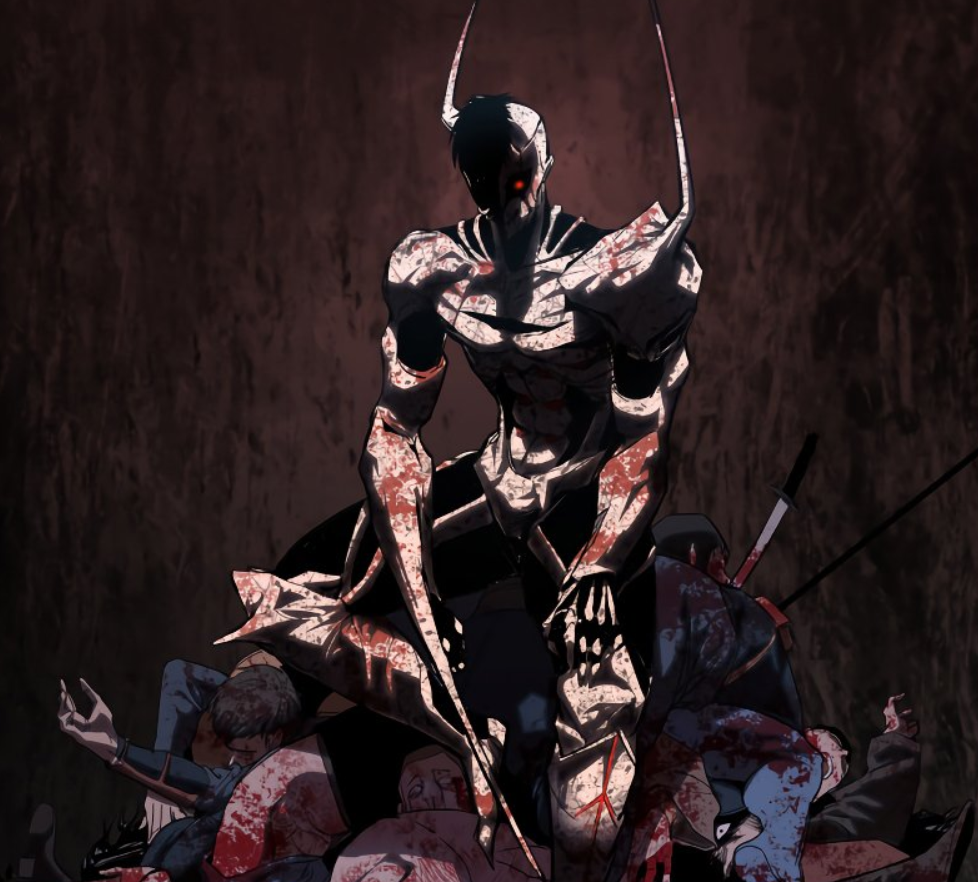
\includegraphics[width=0.5\textwidth]{Bones.png}\\ [1cm]
    \Huge\bfseries}
\posttitle{\end{center}}
\title{Making the solver}
\author{Ojas Ameet Sevekar \\ \textsanskrit{ओजस अमित सेवेकर}}
\date{27/08/2026}

\setlength{\parskip}{0.75em}
\setlength{\parindent}{0pt}
%\setlength{\cftbeforesecskip}{0.5em}   % space before each section entry in toc
\setlength{\cftbeforesubsecskip}{0.5em}
%Colours
\definecolor{sampler}{rgb}{0.63, 0.79, 0.95}
\definecolor{ruler}{rgb}{0.9, 0.6, 0.6}
\definecolor{mathset}{rgb}{0.6, 0.9, 0.6}
\colorlet{intro}{brown}
%New commands and environments
\newcommand*{\bt}[1]{\textbf{#1}}
\newcommand*{\ut}[1]{\uline{#1}}
\newcommand*{\vm}[1]{\boldsymbol{#1}}
\newenvironment{example}{\def\FrameCommand{\colorbox{sampler}} \MakeFramed{\advance\hsize+\width}\begin{center}}{\end{center}\endMakeFramed}
\newenvironment{syntax}{\def\FrameCommand{\colorbox{ruler}} \MakeFramed{\advance\hsize+\width}\begin{center}}{\end{center}\endMakeFramed}
\newenvironment{setdef}{\def\FrameCommand{\colorbox{mathset}} \MakeFramed{\advance\hsize+\width}\begin{center}}{\end{center}\endMakeFramed}

\begin{document}
\begin{titlepage}
\maketitle
\end{titlepage}
\tableofcontents \clearpage

\section{Introduction} \label{sec:enint}
This document gives a brief overview of the methods used to develop the solver. It is not intended to  comprehensively document them, but rather serves as an introduction of the main concepts and design choices that have been made, so as to facilitate other authors to later make their own contributions. In particular, three things are considered:
\begin{enumerate}
\item  Structure of the employed \LaTeX{} code 
\item Naming and usage conventions 
\item GitHub repository structure
\end{enumerate}
Understanding  these things is crucial for those willing  to contribute to any linguistic solution themselves. The resultant standardization  makes it possible to easily update and use the solver, irrespective of how complex and long it may become in the future. 

To begin with, we must look at what \LaTeX{} is and why it matters, especially for creating any such solver. Those interested only in the implementation may skip to \autoref{sec:enstruc}.
\section{Typography and LaTeX} \label{sec:entyp}
Any written language is composed of a visible set of characters placed strategically on a background (like a paper), which is interpreted based on the respective language rules. The placement of these characters must therefore follow certain rules themselves, sometimes out of necessity and other times because things start looking oddly worrisome  if consistency is not maintained:
\begin{example}
The\,end / The\!end / The end
\end{example}
In the above example, the effect of spacing can be observed. The third `The end' looks the most aesthetic, while in the worst case, the second is incorrectly fused and interpreted as a single word. This is merely a tiny glimpse into what is called `typography', which may be defined as the art of placing characters on a screen, so that they look visually consistent (and satisfy whatever purpose they had).

Typography is something that goes unnoticed when done well, but becomes painfully obvious if done incorrectly, which is why every person who wishes to seriously write anything must eventually grapple with it. On computers, this concerns the style of characters, their size, spacing, tilting, weight among others, which collectively come under `font features', where a `font' is the manner in which the alphabet of a script is written. A good overview of \href{https://www.youtube.com/watch?v=BfEvIjTQkIE}{\textcolor{blue}{computer fonts}}.

That being said, the general author normally doesn't want to spend  time wondering about typographical technicalities, which is why computer font files have certain defaults already loaded in them. Apart from this, other things like paragraph spacing, headings, indents, line spacing\ldots also play a role and are similarly handled by the system on its own. For most general purposes, word processors like \textit{Microsoft Word} provide all the basic functions necessary for creating a style-wise consistent document. This convenience is not without sacrifices.

Anyone who has used \textit{MS-Word} knows the pain of formatting finished documents on it. Every element must be manually dealt with, and sometimes causes unexpected behaviour. Dealing with images is difficult, tables can be broken by a page break and cannot have captions, there are no chapter markers in the final pdf, cross referencing another part of the document is not possible, changing fonts requires explicit selection etc. Some of these shortcomings become fatal for longer documents like books, since manually going through everything is often too cumbersome. Sometimes, explanations may reference some section that is far off from the current page, and without a reference link, would force the reader to waste time in scrolling to the necessary page and return.

For the usability of this solver, some things are crucial:
\begin{enumerate}
    \item Font typography and selection per language
    \item Math variables and symbols
    \item Chapter referencing and ease of navigation in the final pdf
    \item Table, Image and Example formatting
    \item Consistent  and layered control of formatting behaviour
\end{enumerate}
Some of these are impossible or cumbersome with  traditional word processors, and I write this after having solved my first three languages on \textit{MS-Word}. However, all of these  goals and more are easily achievable using  \LaTeX.

Put simply, \LaTeX{} is a document typography system that converts plain text files (.txt) into neatly formatted pdf files. For this conversion, it uses its own TeX engine that `compiles' the text file, referred to as the `LaTeX source file', which has the extension `.tex' upon being saved.  Upon its successful compilation, the output pdf along with some other system files are generated. These system files keep track of specific things like  references, chapters, images etc. and  are also used to reduce compilation time for future runs.

Any \LaTeX{} document must be compiled at least twice: Once for generating the system files, and the second time for reading the system files to automatically generate the table of contents or number images and chapters, for example. Editing the source file and compiling again will update the output pdf.

Despite the fact that \LaTeX{} is a document typography system, it is also akin to a programming language, since every stylistic choice that a user makes must be explicitly defined using fixed commands with fixed syntaxes. Commands always start with a backslash, and range from general to specialized, based on how minutely the user wishes to control the formatting. However,  only  a tiny portion of them are directly executable, which are called primitives. Any possible formatting is possible using certain combinations of primitives, but finding the exact combinations for achieving a certain goal requires background on the TeX engine and is  quite tedious.

To circumvent this, \LaTeX{} allows users to define custom commands and group them in a file called a `package', which can be loaded into any source file later. Once a package is loaded, all commands within it become available for that source file. Hence, the pain of finding which combinations of commands achieve some goal was suffered only once by the people who created the package for it. These  warriors, no matter who they are have my thanks.

A \LaTeX{} source file always starts with the declaration of the `document class', after which all necessary packages and user-defined commands (if any) are loaded. `Environments' are regions where the formatting behaviour is different from the rest of the document, and must be explicitly started and ended. The main content of any document always starts in the `\texttt{document}' environment. It is also possible to separate the main source file  into multiple smaller files for easier grouping, all of which can be included into the main file using the `include/input' command. Compilation is consequently only possible for the main file, although all mini-files also have the `.tex' extension.

Now that the general idea of \LaTeX{} is clear,  important specifics of the solver are considered, which will be necessary to  use and especially to update it.
\section{Important packages and Commands} \label{sec:enstruc}
This solver requires the \bt{LuaLaTeX} engine, run on the `\texttt{shell-escape}' mode for successful compilation. \texttt{shell-escape} is necessary for `tikzexternalize'. A brief description of every package used can be directly found in the solver source code where they are loaded, and will not be repeated.

For an author, the most important packages are \texttt{polyglossia} and \texttt{fontspec}, which control the language and font settings respectively. The official documentation for both of these must be referred to when adding a language and/or font that does not yet exist in the solver. Note that it may not always be necessary to define a new font for a new language.
\subsection{Scripts and Fonts} \label{sec:enfont}
Any font is always defined using the \texttt{fontspec} command:
\begin{syntax}
 \verb|\newfontfamily\(script)font{(fontname)}[(options)]|
\end{syntax}
A font should always be defined with its `script' name (all small letters) as defined by \texttt{fontspec} on page 38, and never by language to avoid duplication. In general, a new font should not be defined, unless adding text in a new language using \texttt{polyglossia} language commands causes a compilation failure. The `fontname' is the file name that remains after eliminating everything after the `-' sign including itself.

There are $3$ main options that one must keep in mind while defining a font:
\begin{setdef}
\begin{tabular}{c}
Script = (script),\\\hline ItalicFont = *-Italic,\\\hline BoldItalicFont = *-BoldItalic
\end{tabular}
\end{setdef}
where (script) has the script name as defined by \texttt{fontspec} on page 38. Depending on whether \textit{Italics} and \bt{\textit{BoldItalics}} exists for that font, the options may be deleted. The normal and \bt{bold} options have been globally included along with the `.ttf' font file extension. Hence, for any additional font that is to be added, at least the regular and bold variants of its .ttf font files must be included in the folder `fonts'. For the sake of simplicity and standardization, \texttt{OpenType} variable fonts with the `.otf' extension are not allowed.

By default, this solver uses the `NotoSans' font family, which means that every font name used has the form:
\begin{syntax}
NotoSans + (suffix)
\end{syntax}
\autoref{tab:enfs} shows some suffixes and the scripts they support. All these fonts and more are readily available on \href{https://fonts.google.com/?query=noto+sans+&preview.script=Latn&preview.lang=pl_Latn}{\textcolor{blue}{Google Noto Fonts}}.
\begin{table}[bth]
    \centering
    \begin{tabular}{|m{3cm}|m{6.5cm}|c|}
        \hline \bt{Script} & \bt{Languages} & \bt{Font}\\\hline
        Latin & German, English, French, Polish, Spanish, Italian, Hungarian\ldots & -\\\hline
        Greek & Greek & -\\\hline
        Cyrillic & Russian, Ukrainian\ldots & -\\\hline
        Devanagari & Sanskrit, Hindi, Marathi\ldots & -, Devanagari\\\hline
        Hangul & Korean & KR\\\hline
        Kanji, Hiragana, Katakana & Japanese & SC, (TC)\\\hline
        Hanzi & Chinese & SC, (TC)\\\hline
        Thai & Thai & Thai\\\hline
        Bengali & Bengali & Bengali\\\hline
        Tamil & Tamil & Tamil\\\hline
        Kannada & Kannada & Kannada\\\hline
    \end{tabular}
    \caption{Fonts and the  scripts they support}
    \label{tab:enfs}
\end{table}

Once a font is defined, all languages that use the  script it provides can be displayed in theory. That being said, until the language is actually added using \texttt{polyglossia}, quotation and language based commands are not available. To add a language:
\begin{syntax}
\verb|\setotherlanguage[(options)]{(lang)}|
\end{syntax}
where `lang' is the language name as defined by \texttt{polyglossia} on page 5. If the language name is \textcolor{red}{red}, then there exist additional options for it, which may be found by clicking the corresponding link. The \textit{italic} options are defaults, which may be changed by setting them during definition. If not, the square brackets may be eliminated. 

Note that \textcolor{red}{Babel shorthands} are \ut{\bt{\textit{NEVER}}} to be used. Type Unicode text like \{ä\} directly using the corresponding keyboard, instead of using \{"a\}. 

Language based commands are detailed by \texttt{polyglossia} on page 13 in the `recommended commands' section. These are used to write in the new language inside the \texttt{document} environment:
\begin{example}
\textkorean{양은 달리고 싶어 한다} - \textchinese{这只羊想跑} - \textsanskrit{भेड़ दौड़ना चाहती है।} - \textjapanese{私の村}
\end{example}
Technically, languages using the same script and punctuation styles do not need to be defined separately. If this trick is used, write its name as a \% comment in front of the \verb|\setotherlanguage| whose syntax it borrows, so as to document its existence.

\subsection{Custom styling}
Some definitions are used in the solver as a stylistic choice. These are detailed in \autoref{tab:ensc} and should be used accordingly.
\begin{table}[bth]
\centering
\begin{subtable}{\textwidth}
\centering
\begin{tabular}{|c|m{8cm}|}
	\hline \bt{Custom cmd} & \bt{Function}\\\hline
	\verb|\ut{}| & Underline\\\hline
	\verb|\bt{}| & Bold\\\hline
	\verb|$\vm{}$| & Boldsymbol - Matrix notation. Requires math mode\\\hline
	intro & Keyword for `brown'\\\hline
    \verb|\texttt{}| & Text arguments for math environments\\\hline
\end{tabular}
\end{subtable}
\begin{subtable}{\textwidth}
\centering
\begin{tabular}{|c|m{8cm}|}
\hline \bt{Custom env} & \bt{Function}\\\hline
	\texttt{example} & Blue box for general examples\\\hline
	\texttt{syntax} & Magenta box for patterns / rules\\\hline
	\texttt{setdef} & Green box for complete set definitions / extremely important and comprehensive examples\\\hline
\end{tabular}
\end{subtable}
\caption{Style choices}
\label{tab:ensc}
\end{table}

All custom environments use center alignment by default. Most of the times, it is helpful to use the `\texttt{tabular}' environment inside any such coloured box, with cell control using `m\{(cm)cm\}' as the column option for wrapping. Note that the total width of any table should not exceed 14cm, otherwise text gets uncomfortably close to the box boundary, which causes \LaTeX{} to throw a fit.

Some warnings:
\begin{itemize}
    \item Do not use environments  inside section commands. \begin{example} \verb|\subsection{\begin{Large} Deutsch \end{Large}}| is not allowed!\end{example}
    \item Language appropriate quotations are only applied by using commands like \verb|\enquote{text}| from the \texttt{csquotes} package. The nature of quotation is declared when using \verb|\setotherlanguage| as an [option]
    \item Not all \LaTeX{} warnings need resolution. Exercise discretion
\end{itemize}
\section{File structure and naming conventions}  \label{sec:enncfs}
The resultant \LaTeX{} project includes each language source file separately in the main file using  \verb|\include|. Within each language source, every major section is included using \verb|\input|. For personal use, a user may comment all unnecessary languages in the main file using \%, and compile only for their language of interest, so as to reduce the length of the reference document.

\bt{\ut{Every}} file/folder name in the entire project must  \ut{always} be written in \textit{ASCII}, which practically means English characters only. This restriction is purely computer based, and  avoids potential filename corruption across systems. If any language uses a non-\textit{ASCII} script, its  language source file name  is set as the closest \textit{ASCII} transliteration: \textjapanese{日本語} - `nihongo'. 

Each language source file along with its section subfiles live in a folder with the English name of that language (all small letters). Since the medium language for this solver is English, non-\textit{ASCII} folder names are  impossible. An explanation of \href{https://www.youtube.com/watch?v=vpSkBV5vydg}{\textcolor{blue}{Unicode and ASCII text encoding}}.

Section naming has the convention:
\begin{syntax}
    (Language code) + (Section Keyword) + .tex
\end{syntax}
where both the parts are in small letters. The language code is the \bt{\textit{BCP-47}} tag for any language as defined by \texttt{polyglossia} from page 8 till 12. In case multiple codes exist, only the simplest variant without any `-' sign will be considered. The chapter for any new language will use the same label as its language  code. Section keywords refer to one of the $6$ main sections that occur for any language. These keywords are documented in \autoref{tab:enseckey}.
\begin{table}[bth]
    \centering
    \begin{tabular}{|c|m{8cm}|}
        \hline \bt{Keyword} & \bt{Description}\\\hline
        \texttt{albt} & Alphabets and pronunciation (Optional)\\\hline
        \texttt{noun} & The noun unit and its accessories\\\hline
        \texttt{verb} & The verb chain and its properties\\\hline
        \texttt{prep} & Prepositions\\\hline
        \texttt{stce} & The sentence unit and its modes\\\hline
        \texttt{spco} & Special features unique to the target language\\\hline
        \texttt{rmrk} & Closing remarks and references\\\hline
    \end{tabular}
    \caption{Section keywords}
    \label{tab:enseckey}
\end{table}

So for example,  sections describing  `estonian' would be named as:
\begin{example}
etnoun.tex; etverb.tex; etprep.tex; etstce.tex; etspco.tex; etrmrk.tex
\end{example}
with the chapter itself being labelled: \verb|\label{chap:et}|

In the unlikely event that some language has features that do not fit in any of the above sections, one may create another section file with its own keyword, with the explanation of why it came to be as the very first paragraph in that section.

To standardize the way every section or table is referenced within \LaTeX, the following naming convention has been employed:
\begin{enumerate}
    \item All section reference labels must be named  the same as its file name without the `.tex' extension. Ex: \verb|\label{sec:etnoun}|
    \item Section reference labels must be declared immediately after  \verb|\section|
    \item Subsections or lower do not have reference labels
    \item Tables are named with the section name followed by the letter `T', then the table number 
\end{enumerate}
By table number, I literally mean the order of occurrence, with the first table in a section being numbered `1'. So the third table for `estonian' in section `prep' would have label: \verb|\label{tab:etprepT3}|. Though this may seem inconvenient, there aren't that many important tables in any given section to keep track of. If `tikz' images are involved for any reason, the labelling  should be of the form: \verb|\label{fig:etprepZ3}|

Some minor tips and remarks:
\begin{example}
    \begin{enumerate}
        \item Use \verb|\autoref| to refer to sections and tables
        \item Multiple spaces between words, or a line break are interpreted as a single space by \LaTeX
        \item A new paragraph begins by leaving a blank line between blocks of text
        \item The `Sans' font family in \verb|\setsansfont| is actually loaded as `NotoSerif', since `NotoSans' is the main family
        \item As a rule, assume that neither the `Mono' font for \verb|\texttt| nor the `Serif' font for \verb|\textsf| can deal with non-\textit{ASCII} text
        \item If non-\textit{ASCII} arguments must be provided inside a math environment, use \verb|\text{\text(lang){arg}}|
        \item Section commands like \verb|\subsection| take two arguments: [tableofcontents name], \{Section name\}. No commands are allowed [here], although language switching using \verb|\text(lang)| is fine \{here\}. If \verb|\text(lang)| is used, [needs an argument, which need not be \textit{ASCII}]
        \item The table of contents does not record `subsubsections'
    \end{enumerate}
\end{example}
\section{GitHub repository structure}
\bt{Git} is a version update system that keeps track of files as they are changed, and also of who changed what. It stores the history of all changes and makes it possible to revert any project back to a previous state, allowing for a security net, making it particularly useful for software development. \bt{GitHub} is an online platform based on \bt{Git}, which has been used for storing the solver. This ensures that development can occur from any part of the world, and safeguards the solver against possible mistakes.

Although the net entry barrier for both \bt{GitHub} and \LaTeX{} is high, these are both fantastic open source tools that will be helpful regardless  of what you plan to do in the future. Combined, they have made it possible to  collaborate systematically across the globe: an ability that this solver intends to capitalize on to the fullest. Hence, although this next part can be a headache, please bear with it.
\subsection{Users}
A learner who merely wishes to use the solver need not possess a \bt{GitHub} account. Use the \texttt{Code} tab in the repository,  download the entire thing as a .zip file, and unpack it on your computer. Then, open \texttt{ENG.tex} (the main file) and comment the \verb|\include| lines for languages you don't want (using \%). Thereafter, follow the steps in \autoref{sec:enstruc} and compile the main file. The resultant output pdf is ready to use.
\subsection{Contributors}
Anyone willing to contribute to the solver must own a GitHub account, and be at least bilingual. There are two kinds of contributors for any perspective, and these have different roles to play:
\begin{itemize}
    \item \textit{Primary author}: The one(s) responsible for maintaining the solution for a particular perspective
    \item \textit{Co-authors}: Those who have edited part of the solver. Includes both the ones in it for the long run, and the ones who turn up occasionally
\end{itemize}
The co-authors in it for the long run, as well as the primary author of any perspective (assuming I have been displaced as primary author) will be placed in language teams of all languages they know, as part of the organisation \bt{Ausblicksumwandler}. This means that someone who knows German and French gets placed in both these teams simultaneously if staying for the long run.

The way an update proceeds is as follows:
\begin{enumerate}
    \item Someone proposes a change in some \texttt{(lang)/} path using a pull request. This someone could be anyone from anywhere, and not necessarily a member of the organisation
    \item The teams for the medium and target, in this case `en, (lang)' must review the change. At least one person from both these teams must agree to the change and approve it
    \item After both teams have approved a pull request, I am the one who will approve it last and make it  mergeable  with the \texttt{main} branch. This serves as more of a structural security overview: I do not intend to overly scrutinize and mess with every proposed change (unless you change something I have personally solved)
    \item Team members can also propose changes, which would then need to be approved by someone else from their team. This is because one cannot propose and approve their own change, even if normally authorised to do so. I am not exempt from this process either: Although I hold final merge authority (by virtue of being the final one to approve anything), I cannot and will not merge unless the relevant language teams have already reviewed and accepted my changes
\end{enumerate}
\ut{In the initial phases, as the teams are small, some of the structure may not look exactly like this, but this is the plan.} Please note that although the rules are comprehensive, an approval given by any bilingual normally satisfies both the \texttt{medium/target} team approval conditions simultaneously. Hence, it is important to ensure that no part of the change is accidentally glossed  over.

The method to propose a change is roughly as follows:
\begin{enumerate}
    \item Fork (duplicate) the repository \texttt{Ausblicksumwandler/langsolve-en} on your GitHub account
    \item Download and edit the necessary source files
    \item Compile locally using LuaLaTeX, then debug possible errors and warnings
    \item Create a branch in your fork (with source as the \texttt{main} branch of your fork) and update  the  `.tex' files as a push to it
    \item Create  a Git pull request with base repository  \texttt{Ausblicksumwandler/langsolve-en}, base branch  \texttt{main}, head repository  your fork, and compare branch as the branch you created in your fork. Use appropriate comments in pull requests explaining your changes
    \item Do not worry about file duplication on pushing the edited files into your fork branch, since \bt{GitHub} automatically calculates the changes made and stores the latest file version
    \item Allow maintainers to make changes to the pull request branch, so that everything doesn't need to be done again in case something minor needs  correction
\end{enumerate}
There are some other variations to this: for example one can also work on a pull request started by someone else, but I will spare you the details. Once the change is reviewed, the pull request may be granted, which then truly updates the solver.

The soul of a language embodies the cultures and histories of those who speak it. Whether this soul survives and in what form is completely up to the people involved. A cursed spirit (\textsanskrit{केतु}) like myself can only create  a mechanism to house it, which I will be observing  with great interest.

\begin{center}
    \Large
\textsanskrit{ओजस अमित सेवेकर}
\end{center}
Photo source: Bones - \textkorean{본즈}
\end{document}